%% Ankur Sinha

%% packages %%
% support for coloured text
\usepackage{color}
% IPA
\usepackage{tipa}
\usepackage[scale=2]{ccicons}
\usepackage{amssymb}
\usepackage{tikz}
\usetikzlibrary{mindmap, arrows.meta, positioning, arrows}
\usepackage{pgfplots}
% Define the colours we use for E and I in all graphs
\definecolor{SinhaBlueE}{HTML}{3b4cc0}
\definecolor{SinhaRedI}{HTML}{f7a789}
\pgfmathdeclarefunction{gaussnew}{4}{%nu, eta, eps, omega
  \pgfmathparse{(#1*((2*exp(-(((x-((#2+#3)/2))/((#2-#3)/(2*sqrt(-ln(#4/2)))))^2))) -#4))}%chktex 36
}
\usepackage{jneurosci}
\usepackage{subfig}
\usepackage[T1]{fontenc}
\usepackage[utf8]{inputenc}
\usepackage[style=nature,backend=biber,autocite=footnote]{biblatex}
\addbibresource{/home/asinha/Documents/01_Readables/00_research_papers/bibliography/masterbib.bib}
% Use opensans
% \usepackage[default,scale=0.95]{opensans}
\usepackage[sfdefault]{roboto}
% for strike through
\usepackage[normalem]{ulem}
% links, urls, refs
\definecolor{links}{HTML}{2A1B81}
% Fedora blue for the theme
\definecolor{FedoraBlue}{HTML}{2A1B81}
\usepackage{hyperref}
\hypersetup{colorlinks,linkcolor=Green,urlcolor=links}
% graphics
\usepackage{graphicx}
% algorithm
\usepackage{algorithmic}
\usepackage{textcomp}
\usepackage{wrapfig}
\usepackage{textgreek}
\usepackage{euler}
\usepackage{csquotes}

% beamer theme
% use defaults for theme
\usetheme[numbering=fraction]{metropolis}
\usefonttheme[onlymath]{serif}
\setbeamerfont{footnote}{size=\tiny}
\setbeamerfont{caption}{size=\tiny}
\setbeamercolor{alerted text}{fg=Green}
\setbeamerfont{note page}{size=\small}

% Not needed in metropolis, but in general footnote citation fixes: https://tex.stackexchange.com/questions/44217/how-can-i-stop-footcite-from-hijacking-my-beamer-columns
% how to use multiple references to the same footnote: https://tex.stackexchange.com/questions/27763/beamer-multiple-references-to-the-same-footnote

% Disable footnoterule
\renewcommand{\footnoterule}{}

%% title %%
\title{Investigating structural plasticity in brain networks using computational modelling}
\author[Ankur Sinha]{Ankur Sinha\\PhD candidate\\Biocomputation Research Group\\University of Hertfordshire.}
\date{17/01/2020}

%% document begins %%
\begin{document}


% title frame %%
\begin{frame}
  \titlepage{}
\end{frame}

%% Three slides for 5 minutes seems good
%% So, 30 slides at most for 50 minutes
\section{Context: what and why?}
\begin{frame}[c]{The plastic---but stable---brain: Hebbian/Homeostatic plasticity}
  \pause{}
  \begin{itemize}
    \item \enquote{Neurons that fire together, wire together.}\footnotemark[1]{}
      \pause{}
    \item \enquote{The more things change, the more they stay the same.}\footnotemark[2]{}
  \end{itemize}
  \footnotetext[1]<2->{\fullcite{Hebb1949}}
  \footnotetext[2]<3->{\fullcite{Turrigiano1999}}
\end{frame}
\begin{frame}[c]{Synaptic plasticity: the popular plasticity}
  \begin{itemize}
    \item changes in efficacy of \alert{existing} synapses,
      \pause{}
    \item changes in structure are ignored\footnote[1]{Even though structural changes in spines and boutons underlie modulation of synaptic efficacy.}.
  \end{itemize}
\end{frame}
\begin{frame}[c]{What underlies large scale reorganisation?}
  \begin{itemize}
    \item \fullcite{Rasmusson1982}
  \pause{}
  \scriptsize{
      \item \fullcite{Wall1984}
      \item \fullcite{Merzenich1984}
      \item \fullcite{Calford1988}
      \item \fullcite{Heinen1991}
      \item \fullcite{Rajan1993}
      }
  \end{itemize}
\end{frame}
\begin{frame}[c]{Two theories:}
  \begin{itemize}
    \item \enquote{unmasking} of pre-existing synaptic connections,
      \pause{}
    \item formation of new synapses (\alert{structural plasticity}).
  \end{itemize}
  \footnotetext[1]{\fullcite{Rasmusson1982}}
\end{frame}
\begin{frame}[c]{Imaging confirms structural plasticity in lesion studies}
    \begin{itemize}
      \item \fullcite{Darian-Smith1994}
        \pause{}
        \footnotesize{
      \item \fullcite{Florence1998}
      \item \fullcite{Keck2008}
      \item \fullcite{Keck2011}
      \item \fullcite{Marik2014}
      }
    \end{itemize}
\end{frame}
\begin{frame}[c]{Also confirms structural plasticity in the unlesioned adult brain}
    \begin{itemize}
      \item \fullcite{Holtmaat2005}
        \pause{}
        \footnotesize{
      \item \fullcite{Stettler2006}
      \item \fullcite{Marik2010}
      \item \fullcite{Chen2012}
      \item \fullcite{Villa2016}
      }
    \end{itemize}
\end{frame}
\begin{frame}[c]{So:}
  \begin{itemize}
    \item not only do the strengths of existing synapses change,
    \item \alert{whole synapses are formed and removed.}
      \pause{}
    \item How? Why?
  \end{itemize}
\end{frame}
\begin{frame}[c]{Aim}
  \begin{center}
    \textbf{Simulate a computational model of peripheral lesioning to study the reorganisation process.}
  \end{center}
  \pause{}
  \begin{itemize}
    \item A \alert{computational model} allows us to:
      \begin{itemize}
        \item investigate every entity in the network: variables from neurons, their neurites, all synapses,
        \item modify any parameters to analyse changes in network behaviour: neuronal parameters, synaptic parameters, other network parameters,
        \item run multiple analyses in parallel,
        \item do it in less time than biological experiments\footnote[1]<2->{Simulations take a week each, but that's still faster than a multi-month laboratory experiment.}.
      \end{itemize}
  \end{itemize}
\end{frame}
\section{Methods: How?}
\begin{frame}[c]{Peripheral lesion protocol I:\ topographic mapping}
  \note[item]{The protocol is pretty standard. Here, for a study in the visual cortex, the retinal field of a rat or a mouse is mapped.}
  \begin{columns}
    \begin{column}{0.5\textwidth}
      \centering
      \includegraphics[width=0.8\textwidth]{99_images/keck-1-1a}%chktex 8
    \end{column}
    \begin{column}{0.5\textwidth}
      \centering
      \includegraphics[width=0.8\textwidth]{99_images/keck-1-1c}%chktex 8
    \end{column}
  \end{columns}
  \footnotetext[1]{\fullcite{Keck2008}}
\end{frame}
\begin{frame}[c]{Peripheral lesion protocol II:\ after peripheral lesion}
  \note[item]{Then, a part of the retina is lesioned. This cuts off inputs to a part of the visual cortex, as shown in the first figure. This forms the Lesion Projection Zone (LPZ). By repeated imaging of the region over months, the reorganisation of the network is tracked.}
  \note[item]{Other lesion studies use similar methods: digit removal, whisker trimming, and so on---anything that cuts off projecting activity on to a set of neurons.}
  \begin{figure}[h]
    \centering
    \includegraphics[width=\textwidth]{99_images/keck-1-2c}%chktex 8
  \end{figure}
  \begin{itemize}
    \item Dotted region encloses the Lesion Projection Zone (LPZ)
    \item Inward \enquote{repair}.
  \end{itemize}
    \footnotetext[1]{\fullcite{Keck2008}}
\end{frame}
\begin{frame}[c]{Data gathered from these experiments: summary}
  \note[item]{So, if this a simple schematic, of the regions around the LPZ, this is what we know from these studies.}
  \begin{columns}
    \begin{column}{0.3\textwidth}
      \centering
      \def\radiuscircle{0.6cm}
\begin{tikzpicture}[scale=0.8, transform shape]
  \fill [fill=black, thick, opacity=0.10] (0,0) rectangle ++(5,7.5);
  \node [below, black] at (3.5, 1.0){Other};

  \fill [cyan, opacity=1.0] (2.5, 3.5) circle (3.0*\radiuscircle);
  \draw [cyan, very thick] (1.5, 1.0)--(2.5, 3.5);
  \node [below, cyan] at (1.5, 1.0){Peri LPZ};

  \fill [black, opacity=1.0] (2.5, 3.5) circle (2.0*\radiuscircle);
  \draw [black, very thick] (1.5, 6.0)--(2.5, 3.5);
  \node [above, black] at (1.5, 6.0){LPZ B};

  \fill [green, opacity=1.0] (2.5, 3.5) circle (\radiuscircle);
  \draw [green, very thick] (3.5, 6.0)--(2.5, 3.5);
  \node [above, green] at (3.5, 6.0){LPZ C};

\end{tikzpicture}

    \end{column}
    \pause{}
    \begin{column}{0.6\textwidth}
      \begin{itemize}
        \item Inward repair of network.
        \item Gradual \alert{ingrowth of excitatory synapses} from the peri-LPZ to the LPZ\@.
        \item Gradual \alert{outgrowth of inhibitory synapses} from the LPZ to the peri-LPZ\@.
      \end{itemize}
    \end{column}
  \end{columns}
\end{frame}
\begin{frame}[c]{Cortical spiking network model: 8000 E, 2000 I neurons}
  \begin{figure}[h]
    \def\svgwidth{0.7\textwidth}
    %% Creator: Inkscape inkscape 0.92+devel, www.inkscape.org
%% PDF/EPS/PS + LaTeX output extension by Johan Engelen, 2010
%% Accompanies image file 'schematic.eps' (pdf, eps, ps)
%%
%% To include the image in your LaTeX document, write
%%   \input{<filename>.pdf_tex}
%%  instead of
%%   \includegraphics{<filename>.pdf}
%% To scale the image, write
%%   \def\svgwidth{<desired width>}
%%   \input{<filename>.pdf_tex}
%%  instead of
%%   \includegraphics[width=<desired width>]{<filename>.pdf}
%%
%% Images with a different path to the parent latex file can
%% be accessed with the `import' package (which may need to be
%% installed) using
%%   \usepackage{import}
%% in the preamble, and then including the image with
%%   \import{<path to file>}{<filename>.pdf_tex}
%% Alternatively, one can specify
%%   \graphicspath{{<path to file>/}}
%% 
%% For more information, please see info/svg-inkscape on CTAN:
%%   http://tug.ctan.org/tex-archive/info/svg-inkscape
%%
\begingroup%
  \makeatletter%
  \providecommand\color[2][]{%
    \errmessage{(Inkscape) Color is used for the text in Inkscape, but the package `color.sty' is not loaded}%
    \renewcommand\color[2][]{}%
  }%
  \providecommand\transparent[1]{%
    \errmessage{(Inkscape) Transparency is used (non-zero) for the text in Inkscape, but the package `transparent.sty' is not loaded}%
    \renewcommand\transparent[1]{}%
  }%
  \providecommand\rotatebox[2]{#2}%
  \ifx\svgwidth\undefined%
    \setlength{\unitlength}{841.88976378bp}%
    \ifx\svgscale\undefined%
      \relax%
    \else%
      \setlength{\unitlength}{\unitlength{} * \real{\svgscale}}%
    \fi%
  \else%
    \setlength{\unitlength}{\svgwidth}%
  \fi%
  \global\let\svgwidth\undefined%
  \global\let\svgscale\undefined%
  \makeatother%
  \begin{picture}(1,0.8)(0,-0.1)%
    \put(0,0.05){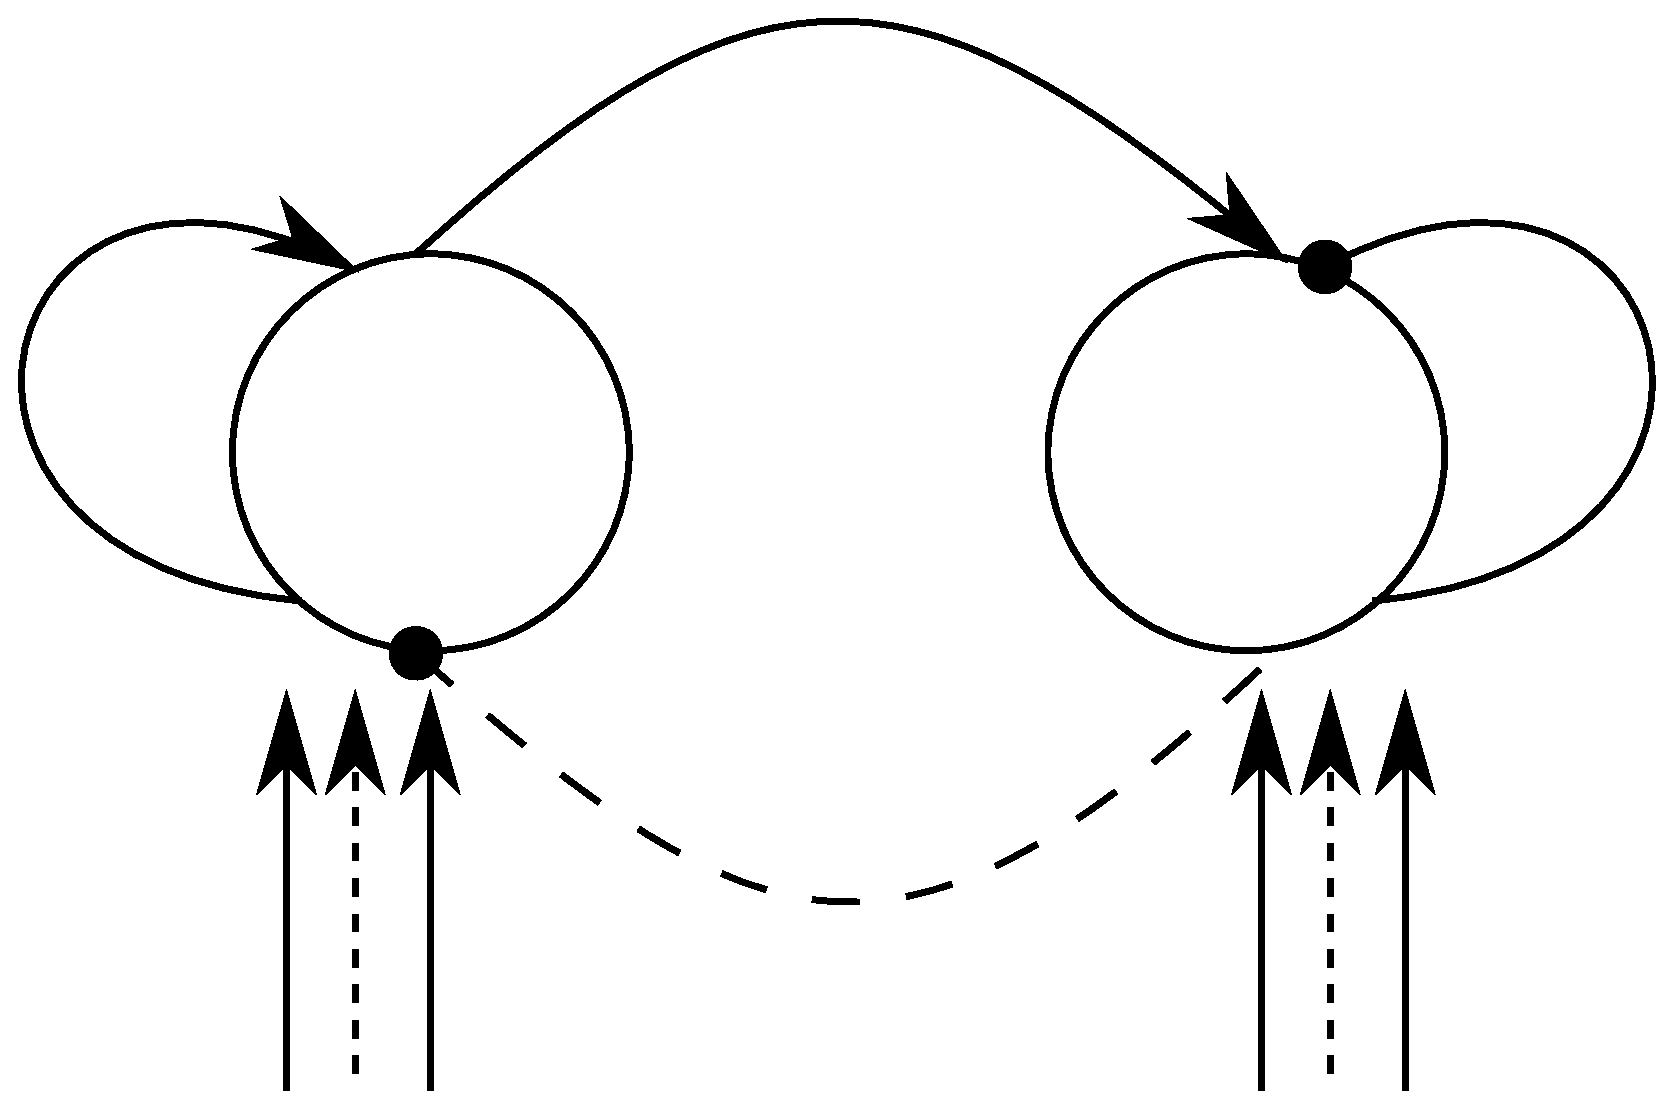
\includegraphics[width=\unitlength]{99_images/schematic.eps}}%
    \put(0.2347176,0.44870591){\color[rgb]{0,0,0}\makebox(0,0)[lb]{\smash{E}}}%
    \put(0.1747176,0.40870591){\color[rgb]{0,0,0}\makebox(0,0)[lb]{\smash{neurons}}}%
    \put(0.73973984,0.44870591){\color[rgb]{0,0,0}\makebox(0,0)[lb]{\smash{I}}}%
    \put(0.66973984,0.40870591){\color[rgb]{0,0,0}\makebox(0,0)[lb]{\smash{neurons}}}%
    \put(0.00355224,0.58941411){\color[rgb]{0,0,0}\makebox(0,0)[lb]{\smash{\(g_{EE}\)}}}%
    \put(0.46685226,0.65011583){\color[rgb]{0,0,0}\makebox(0,0)[lb]{\smash{\(g_{EI}\)}}}%
    \put(0.94063961,0.58941411){\color[rgb]{0,0,0}\makebox(0,0)[lb]{\smash{\(g_{II}\)}}}%
    \put(0.45717629,0.09520415){\color[rgb]{0,0,0}\makebox(0,0)[lb]{\smash{\(\textcolor{Red}{g_{IE}}\)}}}%
    \put(0.05,0.09520415){\color[rgb]{0,0,0}\makebox(0,0)[lb]{\smash{\(g_{ext}^E\)}}}%
    \put(0.86,0.09520415){\color[rgb]{0,0,0}\makebox(0,0)[lb]{\smash{\(g_{ext}^I\)}}}%
    \put(0.08028497,0.00){\color[rgb]{0,0,0}\makebox(0,0)[lb]{\smash{Ext stimulus}}}%
    \put(0.68617882,0.00){\color[rgb]{0,0,0}\makebox(0,0)[lb]{\smash{Ext stimulus}}}%
  \end{picture}%
\endgroup%

\vspace{-0.5cm}
  \end{figure}
  \begin{center}
    Exhibits cortical \alert{Asynchronous Irregular (AI)} firing.
  \end{center}
  \footnotetext[1]{\fullcite{Vogels2011}}
\end{frame}
\begin{frame}[t]{Neuron model}
  \begin{columns}
    \begin{column}{0.6\textwidth}
      \begin{itemize}
        \item Single compartment, point \enquote{leaky integrate and fire neurons}\footnotemark[1]{},
        \item Host neurites (\(z\)).
      \end{itemize}
    \end{column}
    \begin{column}{0.4\textwidth}
      \input{99_images/neuron-str-p.tex}
    \end{column}
  \end{columns}
  \footnotetext[1]{\fullcite{Meffin2004}}
\end{frame}
\begin{frame}[t]{Modelling synapse formation and removal}
  \begin{columns}
    \begin{column}{0.6\textwidth}
      \begin{itemize}
        \item \(z^E_{post} + z^E_{pre}\)
        \item \(z^I_{post} + z^I_{pre}\)
        \item New synapses form when \alert{free} partner neurites are available.
        \item Synapses are deleted if neurites are \alert{retracted} by the neuron.
      \end{itemize}
    \end{column}
    \begin{column}{0.4\textwidth}
      \input{99_images/neuron-str-p.tex}
    \end{column}
  \end{columns}
\end{frame}
\begin{frame}[t]{Neurite growth (\(z\)) as a function of neuronal activity}
  \vspace{0.4cm}
  \begin{columns}
    \begin{column}{0.5\textwidth}
      \centering
      \includegraphics[width=0.9\textwidth]{99_images/lipton1989.png}%chktex 8
    \end{column}
    \pause{}
    \begin{column}{0.5\textwidth}
      \centering
      \begin{itemize}
        \item \([Ca^{2+}]\) correlates with neuronal activity,
        \item serves a homeostatic function.
      \end{itemize}
    \end{column}
  \end{columns}
  \footnotetext[1]{\fullcite{Lipton1989}}
\end{frame}
\begin{frame}[t]{Neurite growth (\(z\)) modelled as a Guassian function of activity}
  \vspace{0.4cm}
  \begin{columns}
    \begin{column}{0.5\textwidth}
      \centering
      \includegraphics[width=0.9\textwidth]{99_images/lipton1989.png}%chktex 8
    \end{column}
    \begin{column}{0.5\textwidth}
      \centering
      \input{99_images/example-gaussian-1.tex}
    \end{column}
  \end{columns}
  \footnotetext[1]{\fullcite{Lipton1989}}
  \footnotetext[2]{\fullcite{Butz2013}}
\end{frame}
\begin{frame}[t]{Growth curves: possibilities}
  \vspace{0.4cm}
  \begin{columns}
    \begin{column}{0.5\textwidth}
      \centering
      \input{99_images/example-gaussian-1.tex}
    \end{column}
    \begin{column}{0.5\textwidth}
      \centering
      \input{99_images/example-gaussian-2.tex}
    \end{column}
  \end{columns}
  \begin{center}
    4 free parameters describe each growth curve. We must determine 6 sets of growth curves: 3 for E, 3 for I neurons.
  \end{center}
  \footnotetext[1]{\fullcite{Sinha2019}}
\end{frame}
\begin{frame}[c]{Replicate peripheral lesion protocol}
  \begin{figure}[h]
    \centering
    \input{99_images/simulation-stages.tex}
  \end{figure}
\end{frame}
\section{Results: a few years later}
\begin{frame}[c]{Reproduction of deafferentation and repair}
  \begin{figure}
      \centering
      \includegraphics[width=0.9\textwidth]{99_images/keck-1-2c}\\%chktex 8
      \quad{}\resizebox{0.9\textwidth}{!}{\input{99_images/201811221433-firing-rate-snapshots-E}}%
  \end{figure}
\end{frame}
\begin{frame}[c]{Reproduction of ingrowth of excitatory projections}
  \begin{figure}
      \centering
      \resizebox{0.9\textwidth}{!}{\input{99_images/201908061027-75-conns-top-EE-lpz_c_E-in}}\\\vspace{0.2cm}%
      \resizebox{0.8\textwidth}{!}{% GNUPLOT: LaTeX picture with Postscript
\begingroup
  \makeatletter
  \providecommand\color[2][]{%
    \GenericError{(gnuplot) \space\space\space\@spaces}{%
      Package color not loaded in conjunction with
      terminal option `colourtext'%
    }{See the gnuplot documentation for explanation.%
    }{Either use `blacktext' in gnuplot or load the package
      color.sty in LaTeX.}%
    \renewcommand\color[2][]{}%
  }%
  \providecommand\includegraphics[2][]{%
    \GenericError{(gnuplot) \space\space\space\@spaces}{%
      Package graphicx or graphics not loaded%
    }{See the gnuplot documentation for explanation.%
    }{The gnuplot epslatex terminal needs graphicx.sty or graphics.sty.}%
    \renewcommand\includegraphics[2][]{}%
  }%
  \providecommand\rotatebox[2]{#2}%
  \@ifundefined{ifGPcolor}{%
    \newif\ifGPcolor{}
    \GPcolortrue{}
  }{}%
  \@ifundefined{ifGPblacktext}{%
    \newif\ifGPblacktext{}
    \GPblacktexttrue{}
  }{}%
  % define a \g@addto@macro without @ in the name:
  \let\gplgaddtomacro\g@addto@macro{}
  % define empty templates for all commands taking text:
  \gdef\gplbacktext{}%
  \gdef\gplfronttext{}%
  \makeatother
  \ifGPblacktext{}
    % no textcolor at all
    \def\colorrgb#1{}%
    \def\colorgray#1{}%
  \else
    % gray or color?
    \ifGPcolor{}
      \def\colorrgb#1{\color[rgb]{#1}}%
      \def\colorgray#1{\color[gray]{#1}}%
      \expandafter\def\csname LTw\endcsname{\color{white}}%
      \expandafter\def\csname LTb\endcsname{\color{black}}%
      \expandafter\def\csname LTa\endcsname{\color{black}}%
      \expandafter\def\csname LT0\endcsname{\color[rgb]{1,0,0}}%
      \expandafter\def\csname LT1\endcsname{\color[rgb]{0,1,0}}%
      \expandafter\def\csname LT2\endcsname{\color[rgb]{0,0,1}}%
      \expandafter\def\csname LT3\endcsname{\color[rgb]{1,0,1}}%
      \expandafter\def\csname LT4\endcsname{\color[rgb]{0,1,1}}%
      \expandafter\def\csname LT5\endcsname{\color[rgb]{1,1,0}}%
      \expandafter\def\csname LT6\endcsname{\color[rgb]{0,0,0}}%
      \expandafter\def\csname LT7\endcsname{\color[rgb]{1,0.3,0}}%
      \expandafter\def\csname LT8\endcsname{\color[rgb]{0.5,0.5,0.5}}%
    \else
      % gray
      \def\colorrgb#1{\color{black}}%
      \def\colorgray#1{\color[gray]{#1}}%
      \expandafter\def\csname LTw\endcsname{\color{white}}%
      \expandafter\def\csname LTb\endcsname{\color{black}}%
      \expandafter\def\csname LTa\endcsname{\color{black}}%
      \expandafter\def\csname LT0\endcsname{\color{black}}%
      \expandafter\def\csname LT1\endcsname{\color{black}}%
      \expandafter\def\csname LT2\endcsname{\color{black}}%
      \expandafter\def\csname LT3\endcsname{\color{black}}%
      \expandafter\def\csname LT4\endcsname{\color{black}}%
      \expandafter\def\csname LT5\endcsname{\color{black}}%
      \expandafter\def\csname LT6\endcsname{\color{black}}%
      \expandafter\def\csname LT7\endcsname{\color{black}}%
      \expandafter\def\csname LT8\endcsname{\color{black}}%
    \fi
  \fi
    \setlength{\unitlength}{0.0500bp}%
    \ifx\gptboxheight\undefined%
      \newlength{\gptboxheight}%
      \newlength{\gptboxwidth}%
      \newsavebox{\gptboxtext}%
    \fi%
    \setlength{\fboxrule}{0.5pt}%
    \setlength{\fboxsep}{1pt}%
\begin{picture}(5760.00,2880.00)%
    \gplgaddtomacro\gplbacktext{%
      \csname LTb\endcsname%
      \put(156,704){\makebox(0,0)[r]{\strut{}\(0.0x10^{0}\)}}%
      \put(156,972){\makebox(0,0)[r]{\strut{}\(1.0x10^{4}\)}}%
      \put(156,1241){\makebox(0,0)[r]{\strut{}\(2.0x10^{4}\)}}%
      \put(156,1509){\makebox(0,0)[r]{\strut{}\(3.0x10^{4}\)}}%
      \put(156,1777){\makebox(0,0)[r]{\strut{}\(4.0x10^{4}\)}}%
      \put(156,2045){\makebox(0,0)[r]{\strut{}\(5.0x10^{4}\)}}%
      \put(156,2314){\makebox(0,0)[r]{\strut{}\(6.0x10^{4}\)}}%
      \put(156,2582){\makebox(0,0)[r]{\strut{}\(7.0x10^{4}\)}}%
      \put(156,2850){\makebox(0,0)[r]{\strut{}\(8.0x10^{4}\)}}%
      \put(744,484){\makebox(0,0){\strut{}\(2.0\)}}%
      \put(1200,484){\makebox(0,0){\strut{}\(2.5\)}}%
      \put(1656,484){\makebox(0,0){\strut{}\(3.0\)}}%
      \put(2112,484){\makebox(0,0){\strut{}\(4.0\)}}%
      \put(2568,484){\makebox(0,0){\strut{}\(6.0\)}}%
      \put(3024,484){\makebox(0,0){\strut{}\(8.0\)}}%
      \put(3479,484){\makebox(0,0){\strut{}\(10.0\)}}%
      \put(3935,484){\makebox(0,0){\strut{}\(12.0\)}}%
      \put(4391,484){\makebox(0,0){\strut{}\(14.0\)}}%
      \put(4847,484){\makebox(0,0){\strut{}\(16.0\)}}%
      \put(5303,484){\makebox(0,0){\strut{}\(18.0\)}}%
    }%
    \gplgaddtomacro\gplfronttext{%
      \csname LTb\endcsname%
      \put(-746,1777){\rotatebox{-270}{\makebox(0,0){\strut{}Synapses}}}%
      \put(3023,154){\makebox(0,0){\strut{}Time (\(x 1000s\))}}%
      \csname LTb\endcsname%
      \put(2564,2707){\makebox(0,0)[r]{\strut{}Other}}%
      \csname LTb\endcsname%
      \put(2564,2487){\makebox(0,0)[r]{\strut{}Peri LPZ}}%
      \csname LTb\endcsname%
      \put(3947,2707){\makebox(0,0)[r]{\strut{}LPZ B}}%
      \csname LTb\endcsname%
      \put(3947,2487){\makebox(0,0)[r]{\strut{}LPZ C}}%
    }%
    \gplbacktext
    \put(0,0){\includegraphics{99_images/201908061027-75-connection-rowstacked-histograms-E-to-lpz_c_E}}%
    \gplfronttext
  \end{picture}%
\endgroup
}%
  \end{figure}
\end{frame}
\begin{frame}[c]{Reproduction of outgrowth of inhibitory projections}
  \begin{figure}
      \centering
      \resizebox{0.9\textwidth}{!}{\input{99_images/201908061027-75-conns-top-IE-p_lpz_E-in}}\\\vspace{0.2cm}%
      \resizebox{0.8\textwidth}{!}{\input{99_images/201908061027-75-connection-rowstacked-histograms-I-to-p_lpz_E}}%
  \end{figure}
\end{frame}
\begin{frame}[c]{Resultant activity dependent growth rules: post-synaptic}
  \begin{columns}
    \begin{column}{0.6\textwidth}
      \centering
      \vspace{0.4cm}
      \input{99_images/growth-curves-den-ours}
    \end{column}
    \pause{}
    \begin{column}{0.5\textwidth}
      \begin{itemize}
        \item E:\ formed when activity is less than, removed when more than optimal.
        \item I:\ formed when activity is more than, removed when less than optimal.
      \end{itemize}
    \end{column}
  \end{columns}\vspace{-0.5cm}
  \pause{}
  \begin{center}
    Neurons attempt to \alert{stabilise their activity} by rebalancing excitatory and inhibitory inputs.
  \end{center}
  \footnotetext[1]<4->{\fullcite{Richards2005}}
  \footnotetext[2]<4->{\fullcite{Knott2002}}
\end{frame}
\begin{frame}[c]{Resultant activity dependent growth rules: pre-synaptic}
  \begin{columns}
    \begin{column}{0.6\textwidth}
      \centering
      \vspace{0.4cm}
      \input{99_images/growth-curves-axonal-ours}
    \end{column}
    \pause{}
    \begin{column}{0.5\textwidth}
      \begin{itemize}
        \item E:\ formed when activity is more than, removed when less than optimal.
        \item I:\ formed when activity is less than, removed when more than optimal.
      \end{itemize}
    \end{column}
  \end{columns}\vspace{-0.2cm}
  \pause{}
  \begin{center}
    Neurons attempt to \alert{project their activity} on to other neurons in the network.
  \end{center}
  \footnotetext[1]<4->{\fullcite{Perez1996}}
  \footnotetext[2]<4>{\fullcite{Schuemann2013}}
\end{frame}
\begin{frame}[c]{Structural and synaptic plasticity are both necessary}
  \begin{itemize}
    \item Only synaptic plasticity: no repair.
      \pause{}
    \item Only structural plasticity: repair, but network does not stabilise; results in high, epileptic firing rates.
      \pause{}
  \end{itemize}
  \begin{center}
  While \alert{structural plasticity} is required for \alert{large scale reorganisation} in synaptic connectivity, \alert{synaptic plasticity} is required to \alert{fine tune} the balance between excitation and inhibition to stabilise the network.
  \end{center}
\end{frame}
\begin{frame}[c]{Results: summary}
  \begin{itemize}
    \item Reproduced peripheral lesion experiments in a computational model.
    \item Suggested testable hypotheses on the activity dependent growth of all neurites.
    \item Proposed that individual neurons may stabilise their activities by modifying their input connectivity.
    \item Indicated that structural and synaptic plasticity both serve distinct roles and are both necessary.
  \end{itemize}
\end{frame}
\begin{frame}[c]{Limitations: summary}
  \begin{itemize}
    \item Point, single compartment neurons: ignore \alert{Calcium compartmentalisation},
    \item No \alert{growth factors} were taken into consideration,
    \item Other plasticity mechanisms\ldots{}
  \end{itemize}
\end{frame}
\section{NeuroFedora: Free Software for Free Neuroscience}
\begin{frame}[c]{Modern neuroscience}
  \begin{itemize}
    \item is \alert{heavily software dependent}.
    \item software is frequently \alert{complex} to install, deploy, maintain, update.
    \item software is \alert{rarely checked for correctness (!)}.
      \pause{}
    \item Neuroscientists hail from \alert{diverse academic backgrounds}.
      \pause{}
    \item Scientists are trying to move towards being more \alert{Open}:
      \begin{itemize}
        \item data, methods, analysis, simulations, publishing, collaboration\ldots{}
      \end{itemize}
  \end{itemize}
\end{frame}
\begin{frame}[c]{Free/Open Source Software vs Open Science}
  \begin{center}
    Users should have the freedom to \alert{share, study, and modify} software\footnotemark[1].\\
    \vspace{1cm}
    \alert{Everyone} should have the freedom to \alert{share, study, and modify} scientific material\footnotemark[2].
  \end{center}
  \footnotetext[1]{\href{https://u.fsf.org/user-liberation}{Free software foundation: fsf.org}}
  \footnotetext[2]{\href{http://opensourceforneuroscience.org/}{Open source for neuroscience: opensourceforneuroscience.org}}
\end{frame}
\begin{frame}[c]{NeuroFedora: volunteer driven initiative}
  \begin{itemize}
    \item Enable \alert{Free/Open science}:
      \pause{}
      \begin{itemize}
        \item provide researchers (end-users):
          \begin{itemize}
            \item ready to use \alert{tested} tools.
          \end{itemize}
          \pause{}
        \item help developers (upstream)
          \begin{itemize}
            \item collect feedback from users.
            \item make software improvements.
            \item implement software development standards.
          \end{itemize}
      \end{itemize}
  \end{itemize}
\end{frame}
\begin{frame}[c]{Current status: software}
  \begin{itemize}
    \item Ready to download ISO for computational neuroscience,
      \pause{}
    \item Plethora of tools ready to install and use:
      \begin{itemize}
        \item \alert{Computational modelling:} NEST, Neuron, Genesis, Brian, LEMS, COPASI\ldots
        \item \alert{Neuroimaging:} dicomanonymiser, dipy, fsleyes, jnifti, mne-bids, nilearn, nistats, octave-dicom, pybids, petlink, pynetdicom\ldots
        \item \alert{Utilities}: \LaTeX{}, the Python science stack, daily use productivity tools\ldots
      \end{itemize}
      \pause{}
    \item \alert{180} tools in queue\footnotemark[1]
  \end{itemize}
  \footnotetext[1]{\url{https://pagure.io/neuro-sig/NeuroFedora/issues}}
\end{frame}
\begin{frame}[c]{Current status: team}
  \begin{itemize}
      \item 15 \alert{volunteers:} mainly Free/Open Source Software enthusiasts.
      \item Limited domain knowledge.
  \end{itemize}
\end{frame}
\begin{frame}[c]{NeuroFedora: links}
  \begin{itemize}
    \item Documentation: \url{https://neuro.fedoraproject.org} 
    \item Blog \url{https://neuroblog.fedoraproject.org} 
    \item IRC channel: \#fedora-neuro on Freenode.net\footnotemark.
    \item Telegram channel: @NeuroFedora\footnotemark.
    \item Mailing list on lists.fedoraproject.org\footnotemark.
  \end{itemize}
  \footnotetext[1]{\href{https://webchat.freenode.net/?channels=\#fedora-neuro}{\#fedora-neuro on Freenode}}
  \footnotetext[2]{\href{https://t.me/NeuroFedora}{@NeuroFedora on Telegram}}
  \footnotetext[3]{\href{https://lists.fedoraproject.org/admin/lists/neuro-sig@lists.fedoraproject.org/}{neuro-sig@lists.fedoraproject.org}}
\end{frame}
\begin{frame}[c]{Search: NeuroFedora}
  \begin{figure}[h]
    \centering
    \includegraphics[keepaspectratio,height=0.5\textheight]{99_images/NeuroFedoraLogo01.png}
  \end{figure}
  \begin{center}
    \url{neuro.fedoraproject.org}
  \end{center}
\end{frame}
\begin{frame}[c]{Sources and license}
  \begin{center}
    \href{https://github.com/sanjayankur31/20200117-KARMA-presentation}{github.com/sanjayankur31/20200117-KARMA-presentation}\vspace{1cm}
    \href{http://creativecommons.org/licenses/by-sa/4.0/}{Creative Commons Attribution-ShareAlike 4.0 International License}
  \end{center}
\end{frame}
\end{document}
